\documentclass[letterpaper,10pt,titlepage]{article}

\usepackage{graphicx}                                        

\usepackage{amssymb}                                         
\usepackage{amsmath}                                         
\usepackage{amsthm}                                          

\usepackage{alltt}                                           
\usepackage{float}
\usepackage{color}

\usepackage{url}

\usepackage{balance}
\usepackage[TABBOTCAP, tight]{subfigure}
\usepackage{enumitem}

\usepackage{pstricks, pst-node}

\usepackage{geometry}
\geometry{textheight=10in, textwidth=7.5in}

% random comment

\newcommand{\cred}[1]{{\color{red}#1}}
\newcommand{\cblue}[1]{{\color{blue}#1}}

\usepackage{hyperref}

\usepackage{textcomp}
\usepackage{listings}

\def\name{D. Kevin McGrath}

%% The following metadata will show up in the PDF properties
\hypersetup{
  colorlinks = true,
  urlcolor = black,
  pdfauthor = {\name},
  pdfkeywords = {cs311 ``operating systems'' files filesystem I/O},
  pdftitle = {CS 311 Project},
  pdfsubject = {CS 311 Project},
  pdfpagemode = UseNone
}

\parindent = 0.0 in
\parskip = 0.2 in

\begin{document}

\section*{Surface Integral}
\hrule

For a scalar function $f$ over a surface parameterized by $u$ and $v$, the surface integral is given by

\begin{eqnarray}
  \Phi =& \int_S f \mathrm{d}a\,\\
       =& \int_S f(u,v) \mathrm{d}u\, \mathrm{d}v
\end{eqnarray}

\section*{Maxwell's Equations}
\hrule

\includegraphics[width=\textwidth]{maxwell.eps}

\end{document}
